% ---------------------------------------------------------------------------
%  Adversarial Manipulation of Explanations in Face Verification
%  HCML bonus project report. IEEE conference format.
%
%  Compile: pdflatex main -> bibtex main -> pdflatex main -> pdflatex main
%  (On Overleaf: press Recompile; pdfLaTeX + BibTeX is the default.)
% ---------------------------------------------------------------------------
\documentclass[conference,10pt]{IEEEtran}
\IEEEoverridecommandlockouts

% --- encoding & fonts ------------------------------------------------------
\usepackage[T1]{fontenc}
\usepackage[utf8]{inputenc}
\usepackage{microtype}

% --- maths, tables, figures ------------------------------------------------
\usepackage{amsmath}
\usepackage{amssymb}
\usepackage{booktabs}
\usepackage{graphicx}
\usepackage{cite}
\usepackage[hidelinks]{hyperref}

% --- shorthand -------------------------------------------------------------
\newcommand{\Linf}{L_\infty}
\newcommand{\dsim}{\Delta s}
\newcommand{\eps}{\varepsilon}
\graphicspath{{figures/}}

% ===========================================================================
\begin{document}

\title{Adversarial Manipulation of Explanations\\ in Face Verification}

\author{\IEEEauthorblockN{Kshitij Parashar}
  \IEEEauthorblockA{Human and Identity Centered Machine Learning Project}}

\maketitle

\begin{abstract}
Saliency maps are offered alongside face verification decisions so that a human reviewer can
inspect the machine's reasoning and catch its mistakes. We ask whether that safeguard can be
defeated: can an imperceptible perturbation to one image of a pair leave the decision intact
while making the explanation misleading? On ElasticFace-Arc and the full LFW benchmark, an
$\Linf \le 4/255$ perturbation preserves the decision on 100\% of 2{,}991 accepted genuine
pairs, holds the similarity score to within $\pm 0.026$, and relocates 75\% of the saliency
map's hot-spots, driving map correlation to 0.236 — enough to defeat an auditor who asks
\emph{which} region is cited as evidence. Evaluated instead with insertion and deletion curves,
which ask whether the newly cited region is itself informative, the attacked map retains 89\%
of its faithfulness across all 2{,}991 pairs: the pixels it now highlights still carry the
match. Directly targeting faithfulness, on a 300-pair subset with a wider score band, closes at
most 21.5\% of the distance to a random-saliency floor — a harder objective on a smaller
population, not a like-for-like comparison with the 89\% figure. Two mechanisms set this
ceiling: redundancy inside the face, where the attack merely swaps one identity-bearing region
for another, and learned invariance outside it, where the model has no gradient to exploit. By
correlation, the standard metric in this literature, this is a successful attack; by
faithfulness, the region it newly cites is still real evidence, not fabricated. Both are true,
and only evaluating both shows which kind of audit the attack actually defeats.
\end{abstract}

\begin{IEEEkeywords}
face verification, explainable AI, adversarial attacks, saliency maps, faithfulness
\end{IEEEkeywords}

% ===========================================================================
\section{Introduction}
\label{sec:intro}

Face recognition is deployed where the consequences of error are severe: border control,
forensic casework, evidence in court. Explainability methods such as
xFace~\cite{knoche2023xface} and xSSAB~\cite{huber2024xssab} are proposed for these settings,
on the argument that a saliency map lets a human auditor verify that the system attended to
the right evidence.

That argument rests on an unexamined premise: that the explanation is trustworthy in a way the
decision is not. A saliency map is another model output computed from the same weights and the
same input, and the adversarial fragility of explanations is established for image
classifiers~\cite{dombrowski2019explanations,heo2019fooling}. If the same holds for
verification, the explanation is not an independent check. It inherits the vulnerability of
the system it audits, while appearing more trustworthy because it is legible.

\textbf{Threat model.} A verification system reports \emph{``same person''} and shows a
saliency map justifying the decision. An adversary who can modify \emph{one} of the two
submitted images adds a perturbation that leaves the decision and the similarity score
essentially unchanged while making the explanation point somewhere misleading. The auditor
sees a normal decision with a fabricated justification. We take the auditor's check to be
regional rather than existential: forensic review contests \emph{which} feature is cited as
matching evidence — eyes, nose bridge, mouth — since that is what gets challenged in court, not
merely whether the map looks face-like in the aggregate. An attack that changes the cited
region already defeats that audit; whether the newly cited region is itself genuine evidence is
a second, stricter question, which Section~\ref{sec:faith} answers with insertion and deletion
rather than correlation. This is realistic wherever image files are submitted and later
reviewed, though not for live camera capture. Note the asymmetry with standard adversarial
attacks on biometrics, which aim to flip the decision: here the decision must survive untouched,
and the explanation alone is under attack.

\textbf{Contributions.} We measure a faithfulness baseline for four explanation methods
against a random-saliency floor (Section~\ref{sec:faith}); build an attack that preserves the
decision on 100\% of pairs while relocating 75\% of saliency hot-spots — defeating region-level
auditing — yet leaves the map 89\% as faithful, meaning it cannot make the newly cited evidence
fabricated (Section~\ref{sec:attack}); diagnose the resulting ceiling as redundancy inside the
face and learned invariance outside it (Section~\ref{sec:ceiling}); and show that correlation,
faithfulness, and reliance are three distinct quantities that this literature conflates into
two, so correlation-only evaluation of explanation attacks is optimistic about the audit that
matters (Section~\ref{sec:discussion}).

% ===========================================================================
\section{Experimental Setup}
\label{sec:setup}

We use ElasticFace-Arc~\cite{boutros2022elasticface}, an iResNet-100 producing 512-d
embeddings, with similarity the cosine of the $L_2$-normalised embeddings. The data is LFW
view-2~\cite{huang2007lfw}: 12{,}000 images forming 6{,}000 pairs in 10 folds of 600, each
fold being 300 genuine pairs followed by 300 imposter pairs. We verified this layout rather
than assuming it, since the labelling determines every downstream number: it separates the two
score distributions at Cohen's $d = 8.32$ against $d \approx 0.01$ for two competing
hypotheses, and holds in all ten folds independently.

Each pair is split into a \emph{probe}, the single image an attack may modify, and a
\emph{reference}, which is never touched, by a seeded per-pair coin flip so that the attacked
image is not systematically image 0. Rather than fixing a
threshold by hand we derive it: the Equal Error Rate is 0.300\% at $\tau = 0.2136$, and every
decision-preservation result is reported additionally at $\mathrm{FMR} = 10^{-1}, 10^{-2},
10^{-3}$, so that no conclusion rests on a single operating point. Under the standard LFW
10-fold protocol the pipeline reaches $99.800\% \pm 0.246\%$, matching the published
ElasticFace-Arc figure (these two numbers use different protocols — one global threshold over
all 6{,}000 pairs for EER, nine folds' worth of per-fold thresholds for the 10-fold figure — so
their implied error counts, about 18 and 12 pairs respectively, need not agree); that can only
come out right if the weights, the preprocessing and the pair labelling are all correct, so it
validates everything downstream. Of the 3{,}000 genuine
pairs, 2{,}991 are accepted at $\tau$ and form the attack population.

As a warm-up we confirmed that the pipeline can \emph{break} a decision before asking it to
preserve one: FGSM~\cite{goodfellow2015fgsm} and I-FGSM~\cite{kurakin2017physical} in both
directions reach 100\% success at $4/255$ with zero failures (Appendix~\ref{app:decision}).

% ===========================================================================
\section{Are the Explanations Faithful to Begin With?}
\label{sec:faith}

A post-attack faithfulness number is meaningless without two reference points: how good the
explanation was initially, and what ``no information'' scores. We measure both first.

We use insertion and deletion curves~\cite{petsiuk2018rise}, adapted to verification. Both
perturb the probe and track cosine similarity to the untouched reference, in the order the
saliency map ranks pixels. \emph{Deletion} replaces the most salient pixels with mid-grey, so
a faithful map destroys the match early and low AUC is good. \emph{Insertion} restores them
over a blurred probe, so a faithful map rebuilds the match early and high AUC is good. We
evaluate four maps over all 6{,}000 pairs: the squared
input-gradient~\cite{simonyan2014saliency}, our implementation of xSSAB~\cite{huber2024xssab},
xFace occlusion~\cite{knoche2023xface}, and uniform noise as the control that supplies the
floor.

\begin{table}[!t]
  \centering
  \caption{Faithfulness Before Any Attack}
  \label{tab:baseline}
  \begin{tabular}{lccc}
    \toprule
    method & deletion AUC $\downarrow$ & insertion AUC $\uparrow$ & gap $\uparrow$ \\
    \midrule
    gradient          & 0.1793 & 0.5597 & \textbf{0.3803} \\
    xFace             & 0.1772 & 0.5287 & 0.3516 \\
    xSSAB (combined)  & 0.1971 & 0.5319 & 0.3349 \\
    \midrule
    random (floor)    & 0.3698 & 0.4806 & 0.1108 \\
    \bottomrule
  \end{tabular}
  \vspace{2pt}
  \parbox{\columnwidth}{\footnotesize Genuine pairs, $n = 3{,}000$. The random row is a floor of
  convenience, not a formal minimum: a maximally unfaithful ranking would order pixels by
  \emph{inverse} saliency rather than uniformly at random, which would sit below 0.3698 and was
  not computed here, so every downstream ``to floor'' percentage in this paper is conservative.
  It is nonetheless the scale against which every later number is read.}
\end{table}

Every real method separates decisively from noise (Table~\ref{tab:baseline}): gradient beats
random at Cohen's $d = 3.44$, an order of magnitude larger than any difference \emph{between}
methods ($d = 0.16$ to $1.14$).

Two findings carry forward. Insertion is a weak discriminator here, since random insertion
already reaches 0.481: restoring any half of the pixels over a blurred baseline recovers most
of the similarity. Headroom is 0.08 for insertion against 0.19 for deletion, so attacks should
be judged on deletion. And imposter pairs are degenerate for this metric, since at a base
similarity of 0.003 there is almost no match evidence to localise, which is why the attack
targets accepted genuine pairs.

% ===========================================================================
\section{The Explanation Attack}
\label{sec:attack}

The attack minimises a single loss, one gradient-descent step per iteration:
\begin{equation}
  \mathcal{L}
  =
  \underbrace{\lambda_{\mathrm{pred}}\,
     \mathrm{relu}\!\bigl(\lvert s - s_0 \rvert - \mathrm{tol}\bigr)}
    _{\text{keep the score where it was}}
  +
  \underbrace{\lambda_{\mathrm{expl}}\,
     \rho\!\bigl(M_{\mathrm{att}}, M_{0}\bigr)}
    _{\text{move the explanation}}
  \label{eq:loss}
\end{equation}
where $s_0$ and $M_0$ are the clean similarity and the clean saliency map and $\rho$ is
Pearson correlation.

Two design choices matter. The decision term is two-sided, penalising the score for moving in
\emph{either} direction rather than merely for falling below a floor, since a one-sided floor
lets the attack push similarity upward and weakens the claim. The explanation term uses
correlation rather than MSE because correlation is scale-invariant: rescaling a map produces a
large MSE while leaving the pattern a reviewer actually sees unchanged. After each step the
perturbation is projected into the $\eps$-ball and shrunk per sample if the score leaves the
band. We run 2{,}991 accepted genuine pairs at $\eps = 4/255$, 40 steps,
$\mathrm{tol} = 0.05$.

\begin{figure*}[!t]
  \centering
  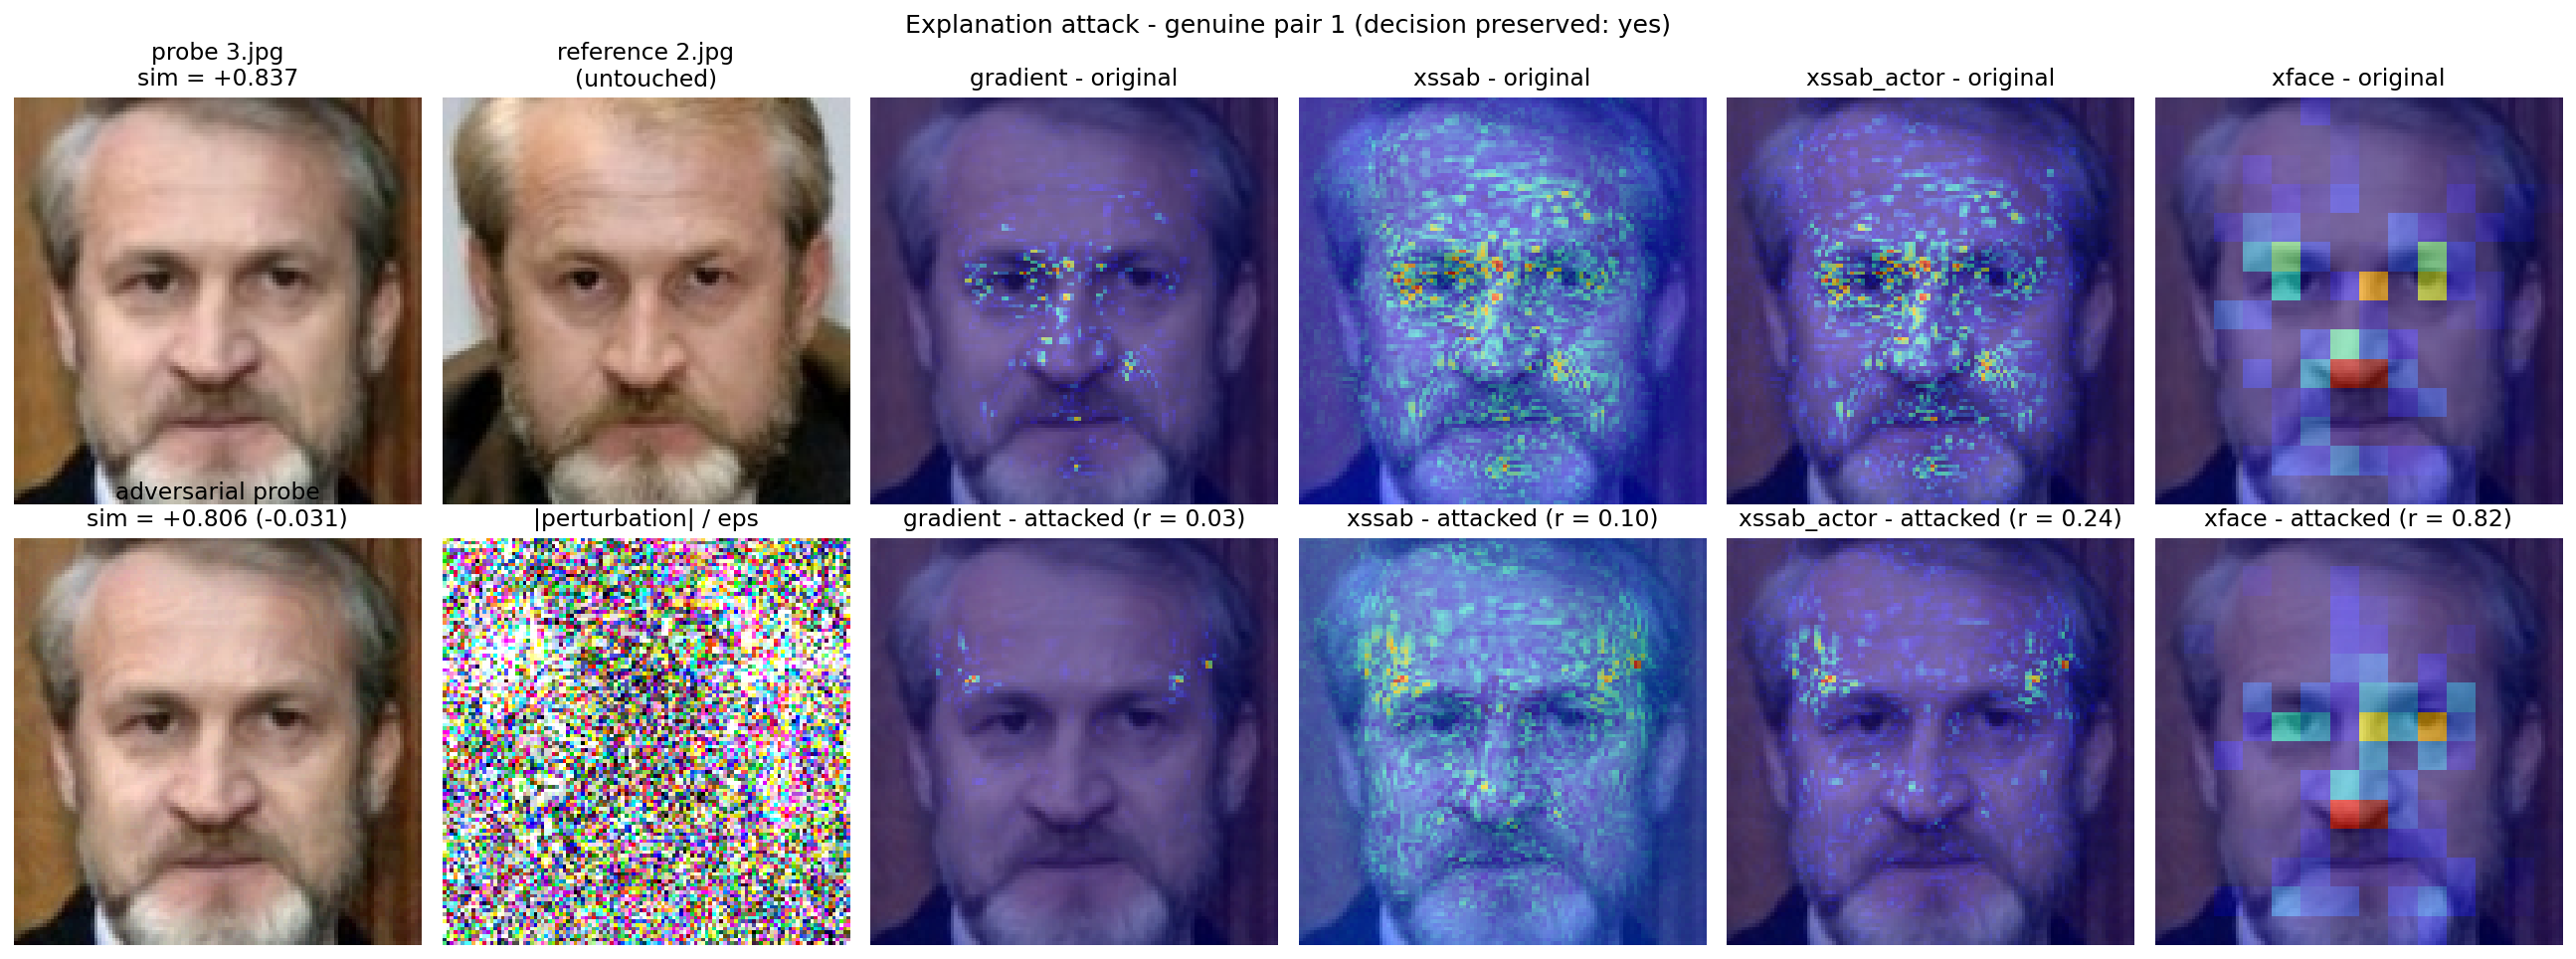
\includegraphics[width=0.62\textwidth]{09_example_pair1.png}
  \caption{The attack on genuine pair 1. Probe \texttt{3.jpg} is modified, reference
  \texttt{2.jpg} is not; the two probe images are indistinguishable and the score moves
  $0.837 \rightarrow 0.806$. Reading the maps left to right shows the transfer staircase
  within a single pair: the targeted gradient map is destroyed ($r = 0.03$), xSSAB partly
  ($r = 0.10$), the actor variant less ($r = 0.24$), and the gradient-free xFace map is
  essentially untouched ($r = 0.82$).}
  \label{fig:example}
\end{figure*}

\textbf{The decision survives.} Mean $\dsim = +0.0110$ and mean $\lvert\dsim\rvert = 0.0261$,
with 95\% of pairs below 0.0474. The decision is preserved on 100\% of pairs at all four
operating points, at a mean $\Linf$ of $2.67/255$. The score does not merely stay on the
correct side of a line; it stays where it was. The positive sign is mildly counter to the naive
prediction from Appendix~\ref{app:decision}, where obfuscation displaces the score \emph{more}
per unit of perturbation than impersonation, which would suggest a negative mean rather than a
positive one; since the two-sided band caps movement in either direction by construction, we
read this as sampling variation within tolerance rather than a directional bias, though we did
not test that directly.

\textbf{The map moves a great deal.} Pearson correlation with the original map falls to 0.236
on average (median 0.128), with 75.7\% of pairs below 0.3, and top-10\% hot-spot overlap is
0.253, so three quarters of the originally hottest pixels relocate. By any map-comparison
metric, the reviewer is shown a different explanation of a decision that has not moved
(Fig.~\ref{fig:example}) — sufficient, under the audit defined in Section~\ref{sec:intro}, to
defeat a reviewer checking which region is cited.

\textbf{But the cited region does not become non-evidence.} Measured by deletion AUC instead
(Table~\ref{tab:attack}), the rise is statistically significant but small: the optimised
gradient map travels only 10.9\% of the distance to the random floor, so it retains 89\% of its
faithfulness. The effect is a real mechanism rather than noise, since per pair the map movement
predicts the faithfulness lost ($r = -0.347$) and the 200 most-disrupted pairs shift nearly
three times the average. The stricter audit — is the cited region real evidence — survives; the
coarser one — which region is cited — does not.

The attack therefore scrambles what the map looks like without substantially destroying what
it knows. Table~\ref{tab:attack} adds a second limitation: correlation after the attack rises
monotonically with distance from the optimised map, from 0.236 for the gradient to 0.720 for
the gradient-free xFace. The attack compromises a \emph{family} of explanations, not the
model's reasoning, so auditing with an occlusion-based tool is a cheap and concrete defence.

\begin{table*}[!t]
  \centering
  \caption{Explanation Metrics Before and After the Attack}
  \label{tab:attack}
  \begin{tabular}{lcccccc}
    \toprule
    & \multicolumn{2}{c}{map similarity (lower $=$ more disrupted)}
    & \multicolumn{4}{c}{faithfulness, deletion AUC (lower $=$ more faithful)} \\
    \cmidrule(lr){2-3}\cmidrule(lr){4-7}
    method & Pearson $r$ & top-10\% IoU & before & after & to floor & retained \\
    \midrule
    gradient (optimised) & \textbf{0.236} & 0.253 & 0.1799 & 0.2007 & 10.9\% & \textbf{89\%} \\
    xSSAB (combined)     & 0.341 & 0.225 & 0.1976 & 0.2232 & 14.9\% & 85\% \\
    xSSAB (actor)        & 0.458 & 0.251 & 0.1801 & 0.2005 & 10.8\% & 89\% \\
    xFace (occlusion)    & \textbf{0.720} & 0.443 & 0.1777 & 0.1952 & \phantom{0}9.1\% & 91\% \\
    \bottomrule
  \end{tabular}
  \vspace{2pt}
  \parbox{0.92\textwidth}{\footnotesize The 2{,}991 accepted genuine pairs. The attack
  optimises the gradient map only, so the map-similarity columns read as a transfer staircase.
  \emph{To floor} is $\Delta\mathrm{del}/(0.3708 - \mathrm{del}_{\mathrm{before}})$, the
  fraction of the distance from the unattacked value to the random-saliency floor, which is
  0.3708 on this population; \emph{retained} is its complement.}
\end{table*}

% ===========================================================================
\section{Why the Attack Has a Ceiling}
\label{sec:ceiling}

Correlation collapses while faithfulness does not, which leaves a gap to explain. Two
hypotheses are testable. \textbf{H1}, the budget: the $\pm 0.05$ band shrank the perturbation
on 49.9\% of pairs, so perhaps the attack was never allowed enough room. \textbf{H2}, the
objective: the attack minimises correlation, but faithfulness is a different quantity, and a
face is redundant. Eyes, nose bridge, mouth and jawline all carry identity, so the attack can
lower correlation by moving the ranking onto a different set of genuinely informative pixels.

\textbf{H1 is real but not sufficient.} Widening the score band (Table~\ref{tab:tol}) buys
genuine disruption, but the marginal returns saturate ($+8.5$, $+6.7$, $+2.5$ points), and at
the widest band the constraint is effectively off: only 2\% of pairs are shrunk, mean $\Linf$
is 3.95 of a 4.00 budget, and correlation is already floored at 0.065. Even there the attack
covers only 21.5\% of the distance to the random floor.

\textbf{H2 is confirmed.} At $\mathrm{tol} = 0.05$, under the border-frame region
(Fig.~\ref{fig:relocation}), off-face saliency mass rises only $0.239 \rightarrow 0.275$,
hot-spots remaining on the face fall only $76.9\% \rightarrow 72.0\%$, and the centre of mass
moves a median of 7.84\,px on a 112\,px image. The mass stayed on the face and moved
\emph{within} it, swapping one identity-bearing region for another, which is why correlation
collapsed while faithfulness did not. (On the border frame's limits as a region definition, see
below.)

\textbf{Attacking faithfulness directly does better, and still hits a wall.} Replacing the
correlation term in (\ref{eq:loss}) with the fraction of saliency mass falling outside the
face lifts the attack from 12.4\% to 15.4\% of the way to the floor ($1.24\times$, $p = 0.014$,
ellipse region), which demonstrates rather than argues that correlation and faithfulness are
dissociable. We lead with the ellipse because it is the defensible region definition: these are
ArcFace-aligned crops~\cite{deng2019arcface} in which the face fills the frame, so the
67.3\%-area border frame (Table~\ref{tab:targetmode}) cuts into the face itself and partly
measures ``not the centre'' rather than ``not the face.'' Under the ellipse, covering 37.8\% of
the image, the unattacked explanation places only 5.3\% of its mass there, a concentration of
0.14 relative to area; the attack quadruples that to 0.215, a concentration of 0.57, well short
of the no-preference level of 1.0. Under the wider, less defensible border frame the same
objective looks far more dramatic — mass rises from 0.239 to 0.614, concentration from 0.36 to
0.91, indistinguishable from no spatial preference at all — yet deletion AUC still closes only
19.9\% of the distance to the floor. The two numbers do not contradict: mass fraction and the
top-decile ranking that deletion AUC actually reads are different statistics, and 61\% of mass
sitting off-face is compatible with the highest-ranked pixels still sitting on the eyes. Either
way, an ArcFace-trained network is invariant to background: the input gradient there is near
zero, so a $\pm 4/255$ perturbation cannot manufacture sensitivity where the model has none.
The attack is fighting a learned invariance, not an optimisation difficulty.

% ===========================================================================
\section{Discussion}
\label{sec:discussion}

Two mechanisms jointly explain the ceiling. Inside the face there is \emph{redundancy}:
multiple regions carry identity, so relocating the ranking among them preserves faithfulness
while destroying correlation. Outside the face there is \emph{invariance}: the model has no
gradient in background, so mass cannot be pushed there. Together they say that the saliency
map's support region is a property of the model, so an imperceptible perturbation can shuffle
mass within that support but cannot move the support itself. This is a positive claim about
robustness rather than a failed attack, and it predicts a structural ceiling on any model
combining background invariance with a redundant signal.

The methodological consequence is the more important result, and it is sharper than a
two-metric contrast. Three distinct quantities are at stake, and this literature conflates them
into two. Correlation measures whether the map \emph{changed}. Deletion and insertion measure
whether the pixels it now highlights are \emph{informative}. Neither measures whether the model
\emph{relied on} those pixels for this decision — and the redundancy finding above is precisely
what puts that third quantity out of reach for any region-based metric here: if several regions
carry identity, a map that relocates onto a different but still-informative region scores as
faithful by deletion regardless of which region the model actually used. With correlation as
the only metric, this study would have reported a successful attack at $r = 0.236$; insertion
and deletion show that the newly cited region, though relocated, is not fabricated. Under the
audit defined in Section~\ref{sec:intro} — which region is cited — the attack succeeds; under
the stricter audit deletion AUC approximates — is the cited region real evidence — it does not.
Both readings are correct simultaneously, because they answer different questions.

This dissociation is demonstrated on one system. Face verification is unusually favourable
ground for it: ArcFace-aligned crops have almost no background, and identity is redundantly
coded across the face, both of which push deletion AUC and correlation apart.
Dombrowski~et~al.~\cite{dombrowski2019explanations} and Heo~et~al.~\cite{heo2019fooling}
establish explanation fragility on image classifiers using correlation-style metrics alone;
whether their attacks also survive an insertion/deletion check is the natural replication
before treating ``correlation-only evaluation is optimistic'' as a general lesson rather than a
property of redundant, background-invariant systems like this one. We did not run that
replication here.

\textbf{Limitations.} The attack is white-box and digital only, with no cross-model transfer
and no JPEG or print-scan robustness; LFW is near-saturated for ElasticFace-Arc; xSSAB is our
implementation rather than the official code; insertion and deletion perturb inputs
off-distribution, a confound the random control bounds but does not remove; only accepted
genuine pairs were attacked; and, as above, the correlation/faithfulness dissociation is shown
on one domain. The clearest next step is therefore a classifier replication of
Dombrowski's~\cite{dombrowski2019explanations} or Heo's~\cite{heo2019fooling} attack under the
same insertion/deletion protocol, since it is the cheapest experiment that would tell us
whether this lesson generalises; a multi-method attack optimising against gradient, xSSAB and a
differentiable occlusion surrogate at once, testing whether the occlusion defence survives, is
the natural follow-up after that.

% ===========================================================================
\section{Conclusion}

An imperceptible perturbation to one image of a pair holds the decision and the score fixed
while rewriting three quarters of the saliency map's hot-spots. That defeats an auditor who
checks which region is cited as evidence — the standard reading in this literature, and the one
map correlation measures. It does not defeat an auditor who checks whether the cited region is
real evidence: by insertion and deletion, the newly cited region remains genuinely informative,
because the saliency map's support is a property of the model rather than of the input, and an
imperceptible perturbation can shuffle mass within that support but not move it. The attack is
narrower than a correlation-only reading would suggest; the audit it leaves intact is the one
worth building.

\bibliographystyle{IEEEtran}
\bibliography{refs}

% ===========================================================================
\appendices
\section{Protocol and Decision Attacks}
\label{app:decision}

Before claiming that an attack \emph{preserves} a decision, the pipeline must be able to
\emph{break} one on purpose. Running FGSM and I-FGSM in both directions over all 6{,}000
pairs, at $4/255$ with I-FGSM both directions reach 100\% with zero failures, with mean
$\dsim$ of $-1.116$ and $+0.691$ respectively. Success holds at approximately 100\% at every
operating point from $\mathrm{FMR} = 10^{-1}$ to $10^{-3}$.

An asymmetry appears at low budget: impersonation succeeds on 62.4\% of pairs at $1/255$
against only 6.7\% for obfuscation. Two competing effects produce this. Obfuscation displaces
the score \emph{more} per unit of perturbation ($1.18\times$ at $1/255$, rising to
$1.73\times$ at $8/255$), since pushing an embedding away from a point is easier than steering
it toward one. But obfuscation also has $2.41\times$ further to travel, because
$\tau = 0.2136$ sits close to the imposter mean (gap 0.210) and far from the genuine mean
(gap 0.506). The second effect dominates. Attack success rates are therefore as much a
statement about where the operating threshold sits as about the attack itself, which is why
the threshold had to be derived before any of this could be interpreted.

\begin{figure}[!t]
  \centering
  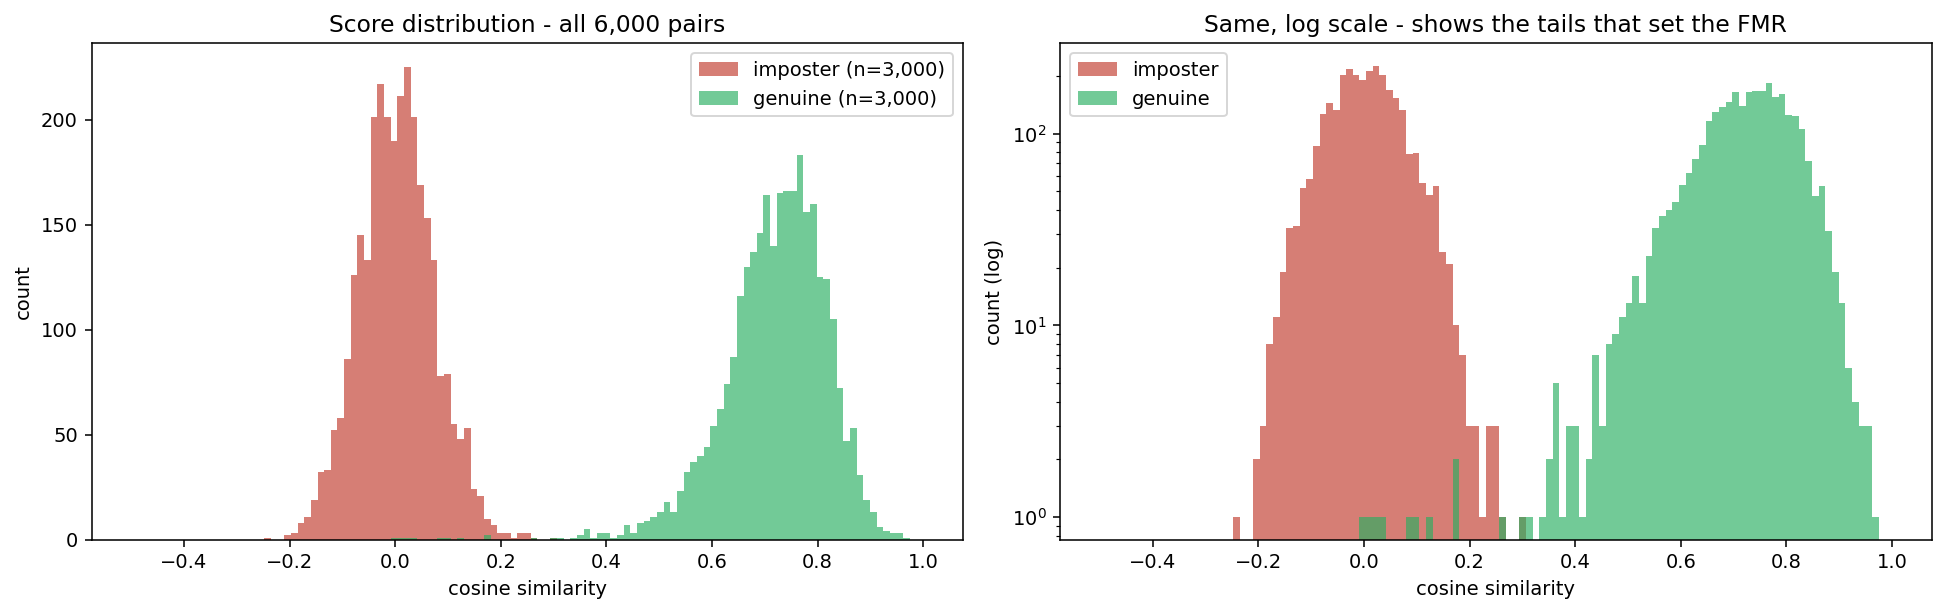
\includegraphics[width=\columnwidth]{06_score_distributions.png}
  \caption{Genuine (green) and imposter (red) cosine-similarity distributions over all 6{,}000
  pairs, linear and log scale. The log panel is the one that matters: with 3{,}000 imposter
  scores the tail is resolved well enough to estimate a false match rate, which the commonly
  used 900-pair subset could not support.}
  \label{fig:scores}
\end{figure}

\begin{figure}[!t]
  \centering
  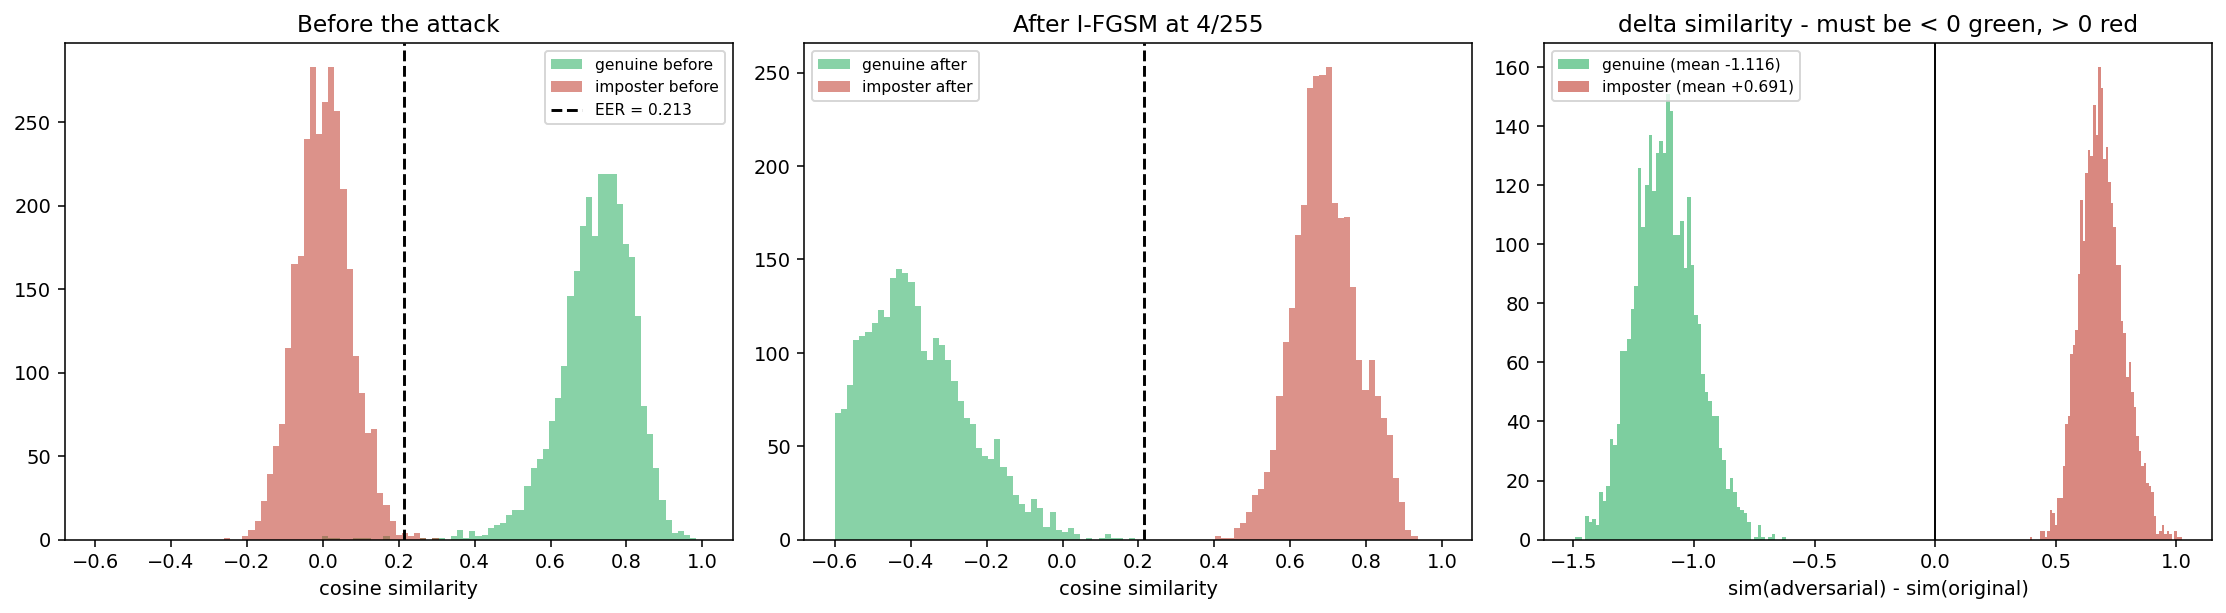
\includegraphics[width=\columnwidth]{08_decision_attack_distributions.png}
  \caption{I-FGSM at $4/255$. The two populations swap sides of the threshold completely. The
  right panel is the direction check: genuine $\dsim$ must be negative and imposter positive,
  and the two distributions do not overlap zero.}
  \label{fig:decision}
\end{figure}

\begin{figure}[!t]
  \centering
  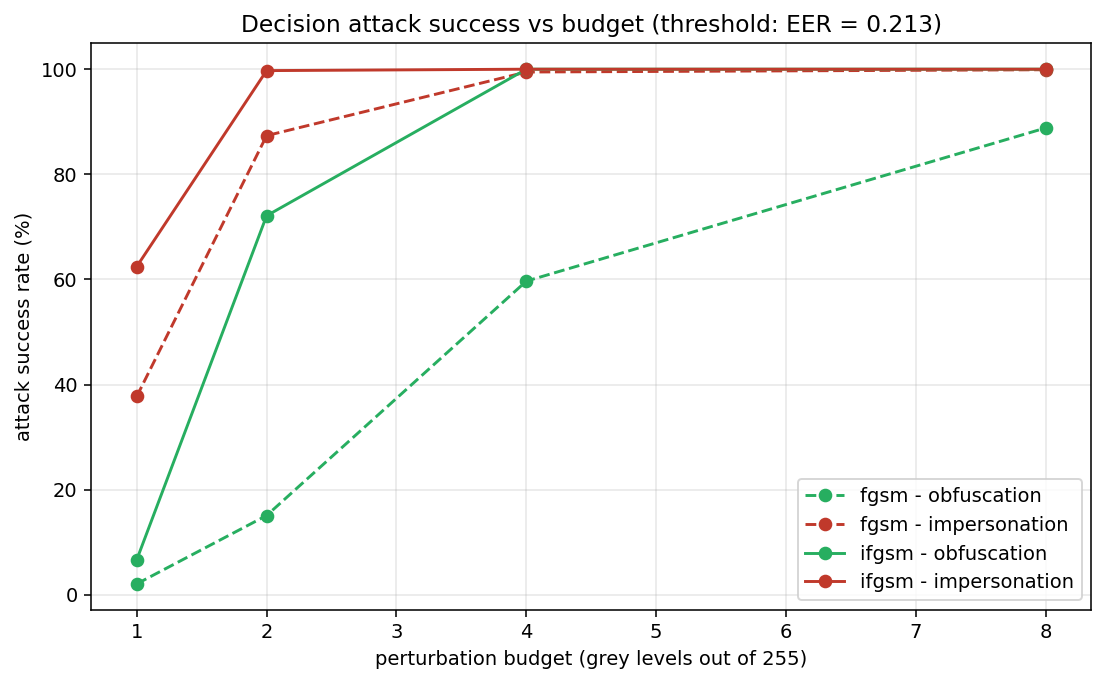
\includegraphics[width=0.82\columnwidth]{08_epsilon_sweep.png}
  \caption{Success rate against budget at the EER threshold. Impersonation (red) dominates at
  small budgets despite obfuscation displacing the score further per unit of $\eps$, because
  the threshold sits closer to the imposter distribution. Both saturate at $4/255$.}
  \label{fig:epssweep}
\end{figure}

\section{Explanation Faithfulness}
\label{app:faith}

\textbf{An aside on xSSAB.} Measuring both variants shows that the actor map alone scores
deletion 0.1801 and insertion 0.5613, identical to the raw input-gradient map, while the
combined actor minus counteractor map is clearly worse (0.1976 / 0.5334). Any ranking that
places xSSAB last is an artefact of scoring the combined map; the actor variant is the one to
use.

\begin{figure*}[!t]
  \centering
  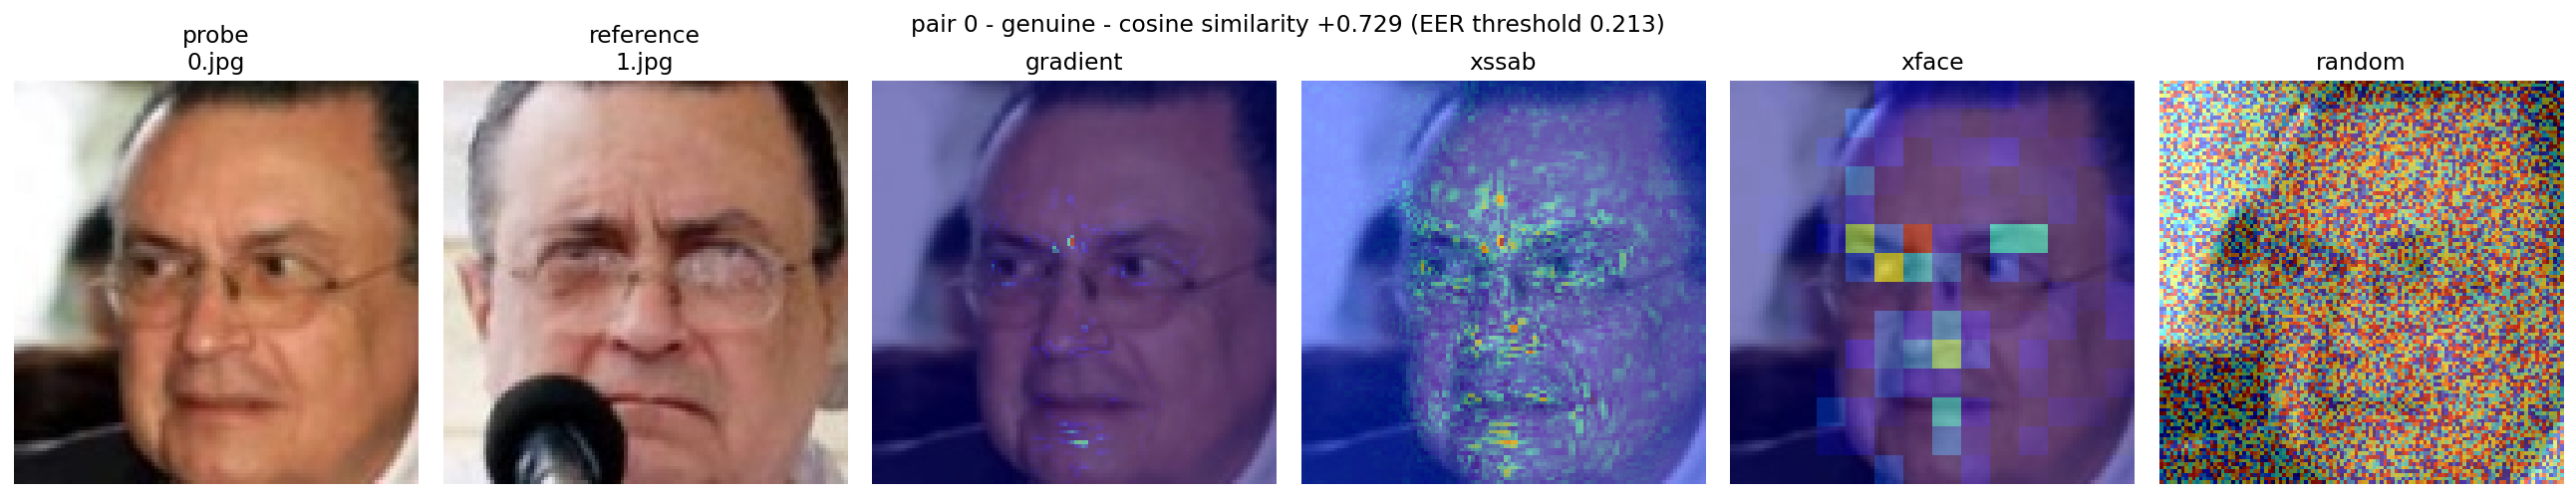
\includegraphics[width=0.94\textwidth]{07_methods_pair0.png}
  \caption{The four maps on genuine pair 0 (similarity $+0.729$). Gradient is pixel-sharp and
  sparse, xSSAB denser and more semantic, xFace blocky because it is grid-based, and the
  random control structureless. All three real methods concentrate on the face interior.}
  \label{fig:methods}
\end{figure*}

\begin{figure}[!t]
  \centering
  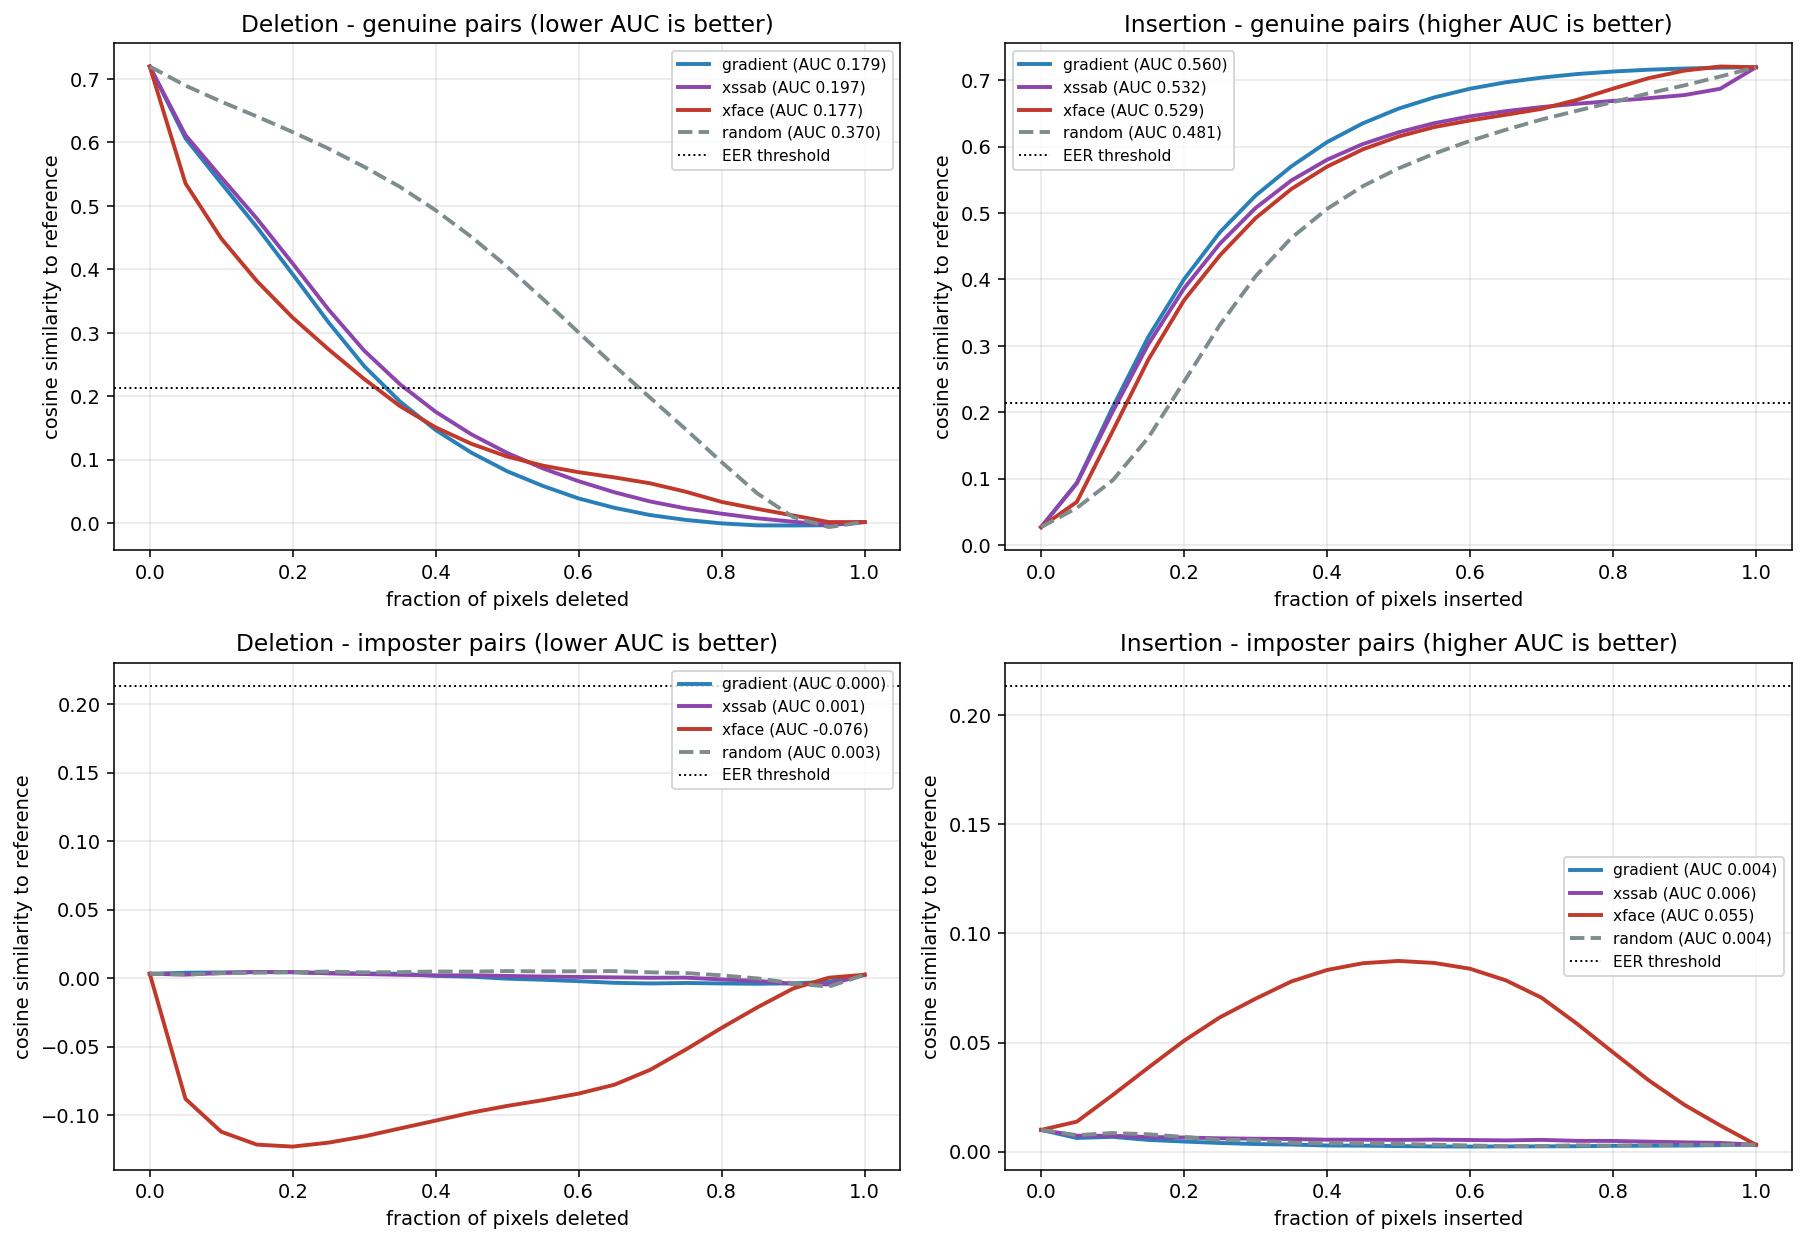
\includegraphics[width=\columnwidth]{07_insertion_deletion_curves.png}
  \caption{Mean insertion and deletion curves over all 6{,}000 pairs, genuine (top) and
  imposter (bottom). For genuine pairs every real method drops far faster than random under
  deletion and rises faster under insertion. The imposter row shows the degeneracy noted in
  Section~\ref{sec:faith}: with almost no match evidence to localise, all curves collapse
  toward zero. xFace is the informative exception, its deletion AUC going negative ($-0.076$)
  because it correctly identifies the few regions supplying positive evidence.}
  \label{fig:insdel}
\end{figure}

\section{Attack Diagnostics}
\label{app:attack}

This appendix collects the sweeps behind Section~\ref{sec:ceiling}'s H1/H2 analysis: the
score-band sweep motivating H1 (Table~\ref{tab:tol}), the region-definition comparison for the
direct faithfulness objective (Table~\ref{tab:targetmode}), and the corresponding per-pair
figures.

\begin{table}[!t]
  \centering
  \caption{Score-Band Sweep}
  \label{tab:tol}
  \setlength{\tabcolsep}{4.5pt}
  \begin{tabular}{cccccc}
    \toprule
    tol & mean $\lvert\dsim\rvert$ & shrunk & Pearson $r$ & del.\ AUC & to floor \\
    \midrule
    0.02 & 0.0118 & 88\% & 0.479 & 0.1983 & \phantom{0}3.9\% \\
    0.05 & 0.0260 & 44\% & 0.220 & 0.2135 & 12.4\% \\
    0.10 & 0.0462 & 14\% & 0.109 & 0.2254 & 19.1\% \\
    0.20 & 0.0606 & \textbf{2\%} & \textbf{0.065} & 0.2298 & \textbf{21.5\%} \\
    \bottomrule
  \end{tabular}
  \vspace{2pt}
  \parbox{\columnwidth}{\footnotesize A 300-pair subset with its own unattacked baseline
  (deletion AUC 0.1915) and floor (0.3698), so \emph{to floor} is not directly comparable with
  Table~\ref{tab:attack}. The $\mathrm{tol} = 0.05$ row is the configuration used in
  Section~\ref{sec:attack}. \emph{Shrunk} is the fraction of pairs whose perturbation the band
  pulled back below the budget.}
\end{table}

\begin{table*}[!t]
  \centering
  \caption{Attacking Faithfulness Directly}
  \label{tab:targetmode}
  \begin{tabular}{lccccc}
    \toprule
    off-face region & area & mass & concentration & to floor & vs.\ decorrelation \\
    \midrule
    border frame & 67.3\% & $0.239 \rightarrow 0.614$ & $0.36 \rightarrow 0.91$ & 19.9\% &
      $1.61\times$, $p = 5.6\!\times\!10^{-9}$ \\
    ellipse (background) & 37.8\% & $0.053 \rightarrow 0.215$ & $0.14 \rightarrow 0.57$ &
      15.4\% & $1.24\times$, $p = 1.4\!\times\!10^{-2}$ \\
    \bottomrule
  \end{tabular}
  \vspace{2pt}
  \parbox{0.92\textwidth}{\footnotesize The same 300 pairs and score band as
  Table~\ref{tab:tol}. Mass and concentration are given as before $\rightarrow$ after;
  concentration is mass share divided by area share, so 1.0 means no spatial preference. The
  decorrelation objective reaches 12.4\% of the way to the floor on this subset.}
\end{table*}

\begin{figure}[!t]
  \centering
  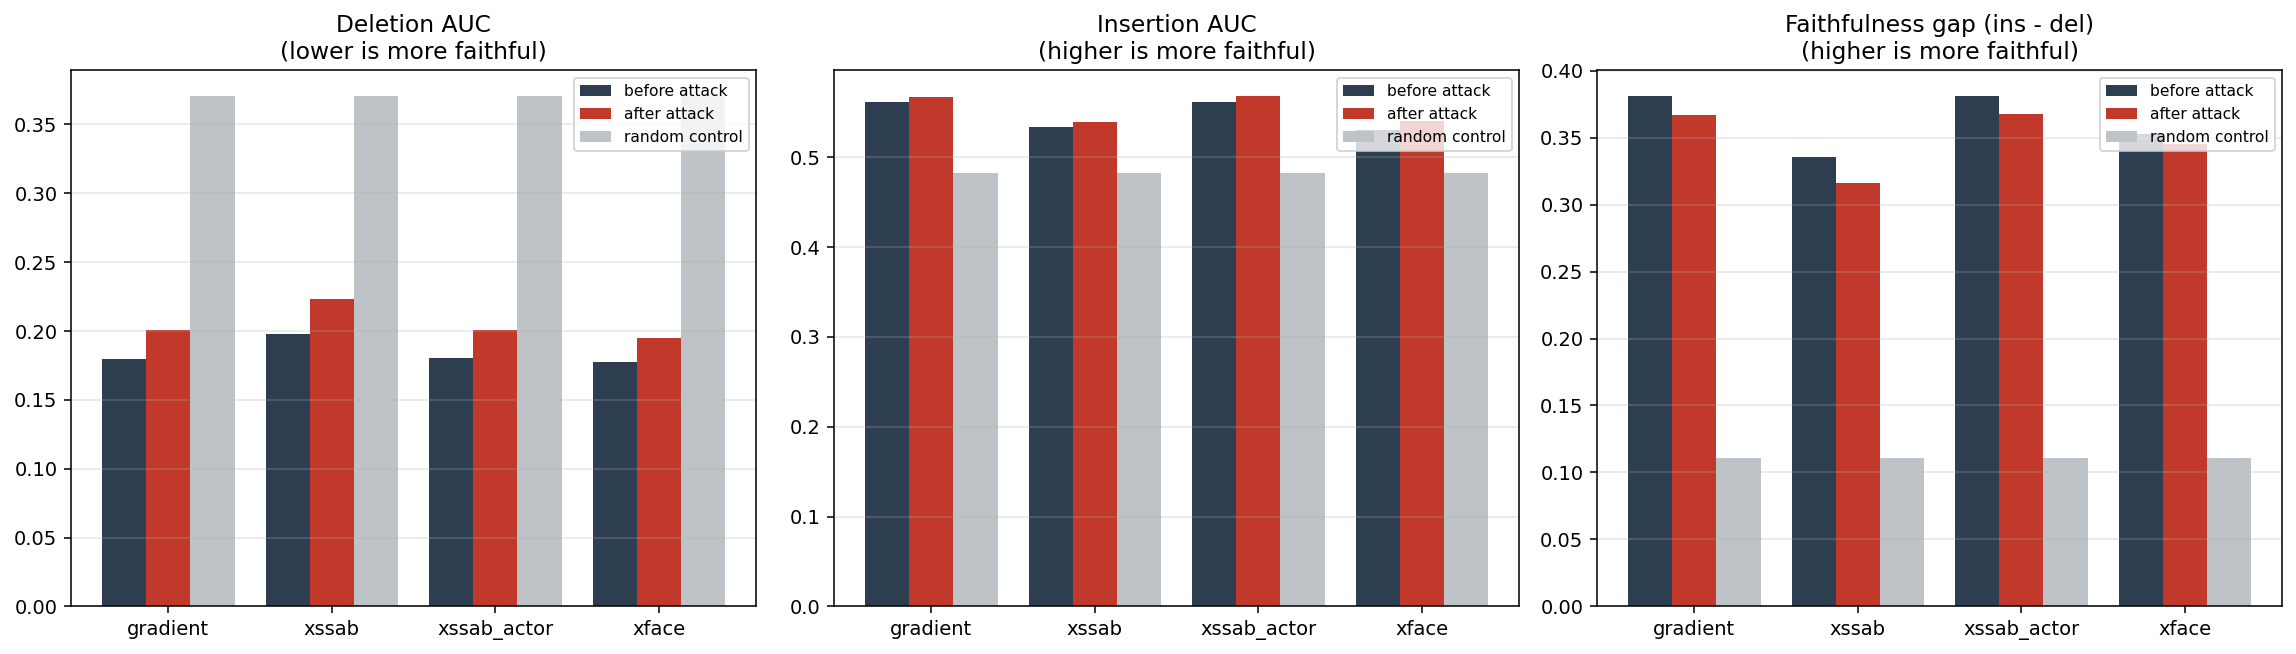
\includegraphics[width=\columnwidth]{10_faithfulness_before_after.png}
  \caption{Faithfulness before (dark) and after (red) the attack, against the random-saliency
  control (grey). The attacked bars barely move from the unattacked ones and remain far from
  the control: the explanation changed, but it did not become uninformative. Insertion
  (middle) moves so little that it is visually flat, consistent with its narrow headroom.
  These are the numbers of Table~\ref{tab:attack} in graphical form.}
  \label{fig:central}
\end{figure}

\begin{figure}[!t]
  \centering
  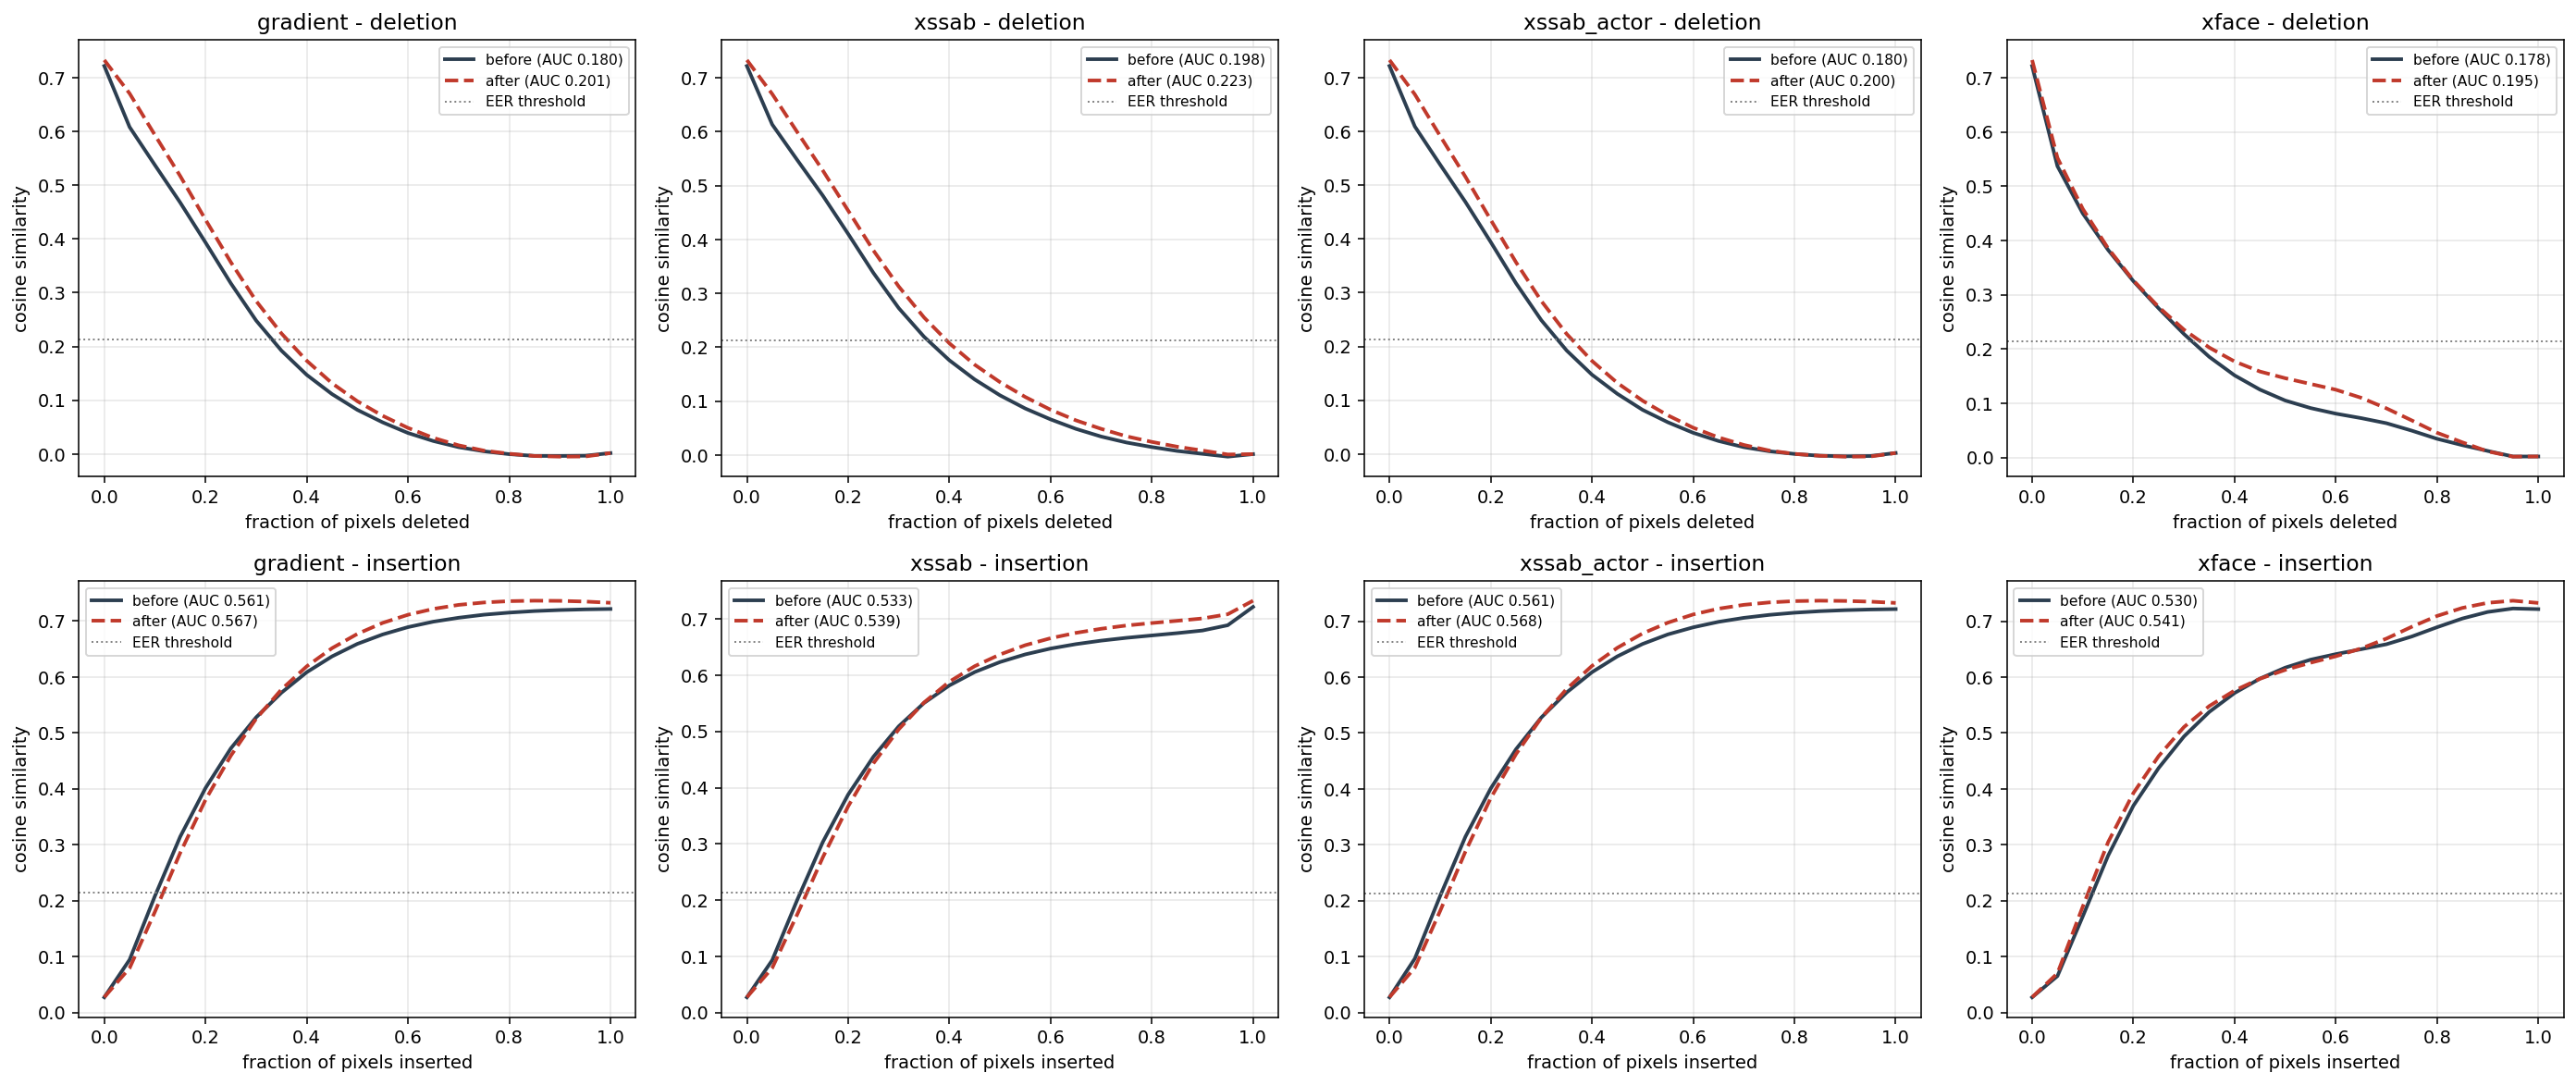
\includegraphics[width=\columnwidth]{09_insdel_before_after.png}
  \caption{The main result as curves rather than areas. The attacked deletion curves (dashed
  red) sit only slightly above the unattacked ones (solid), and the gap closes entirely past
  roughly 60\% of pixels deleted. A successful attack would have lifted the dashed curve
  toward a straight diagonal.}
  \label{fig:curvesba}
\end{figure}

\begin{figure}[!t]
  \centering
  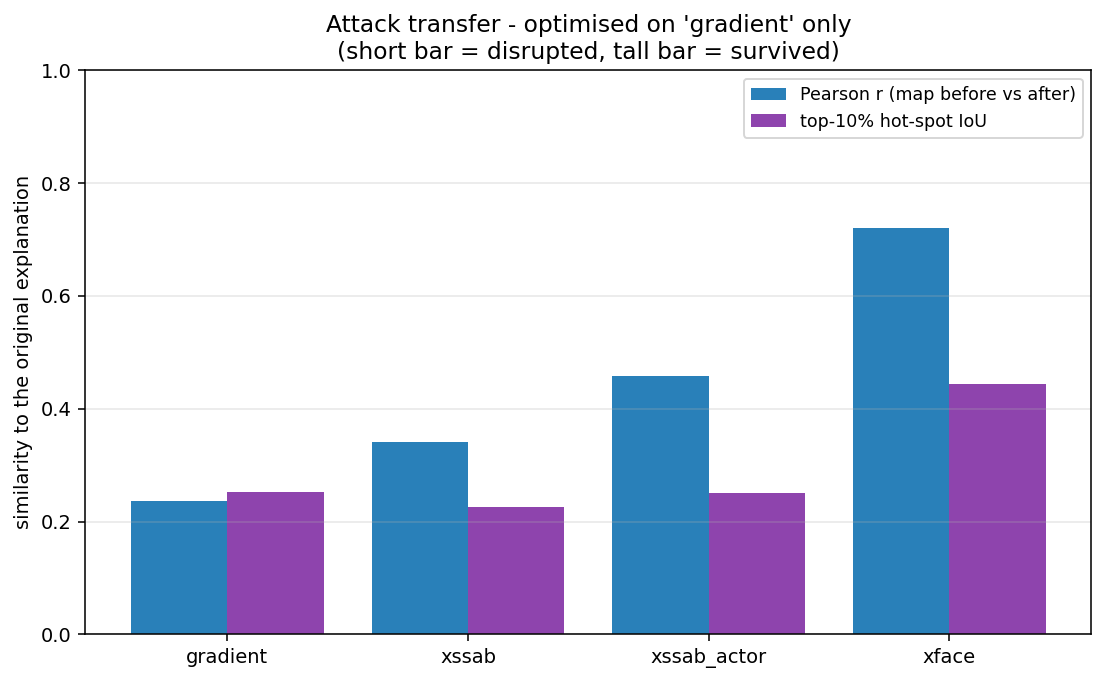
\includegraphics[width=0.82\columnwidth]{10_transfer.png}
  \caption{Transfer. Both map-similarity metrics rise monotonically with distance from the
  optimised map, and xFace, which uses no gradients, retains most of its explanation under
  both.}
  \label{fig:transfer}
\end{figure}

\begin{figure}[!t]
  \centering
  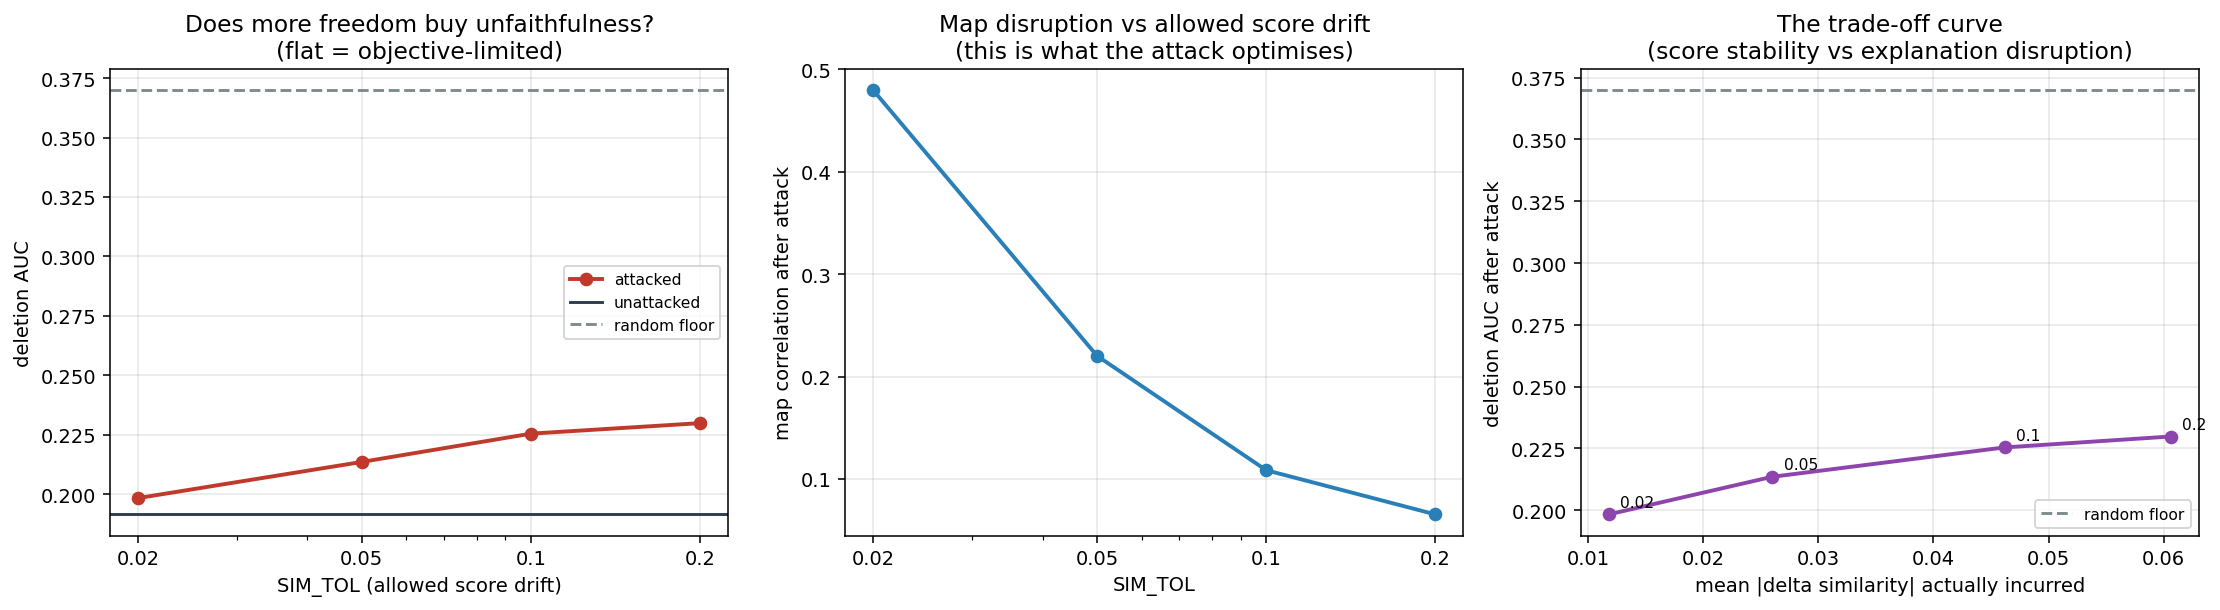
\includegraphics[width=\columnwidth]{11_simtol_sweep.png}
  \caption{Score-band sweep. Left: deletion AUC against the allowed score drift, with the
  unattacked level and the random floor marked; the curve rises but flattens and never
  approaches the floor. Middle: the quantity the attack actually optimises falls steadily to
  0.065, so it is not the correlation objective failing to converge. Right: the trade-off
  curve between score stability and explanation disruption.}
  \label{fig:tolsweep}
\end{figure}

\begin{figure}[!t]
  \centering
  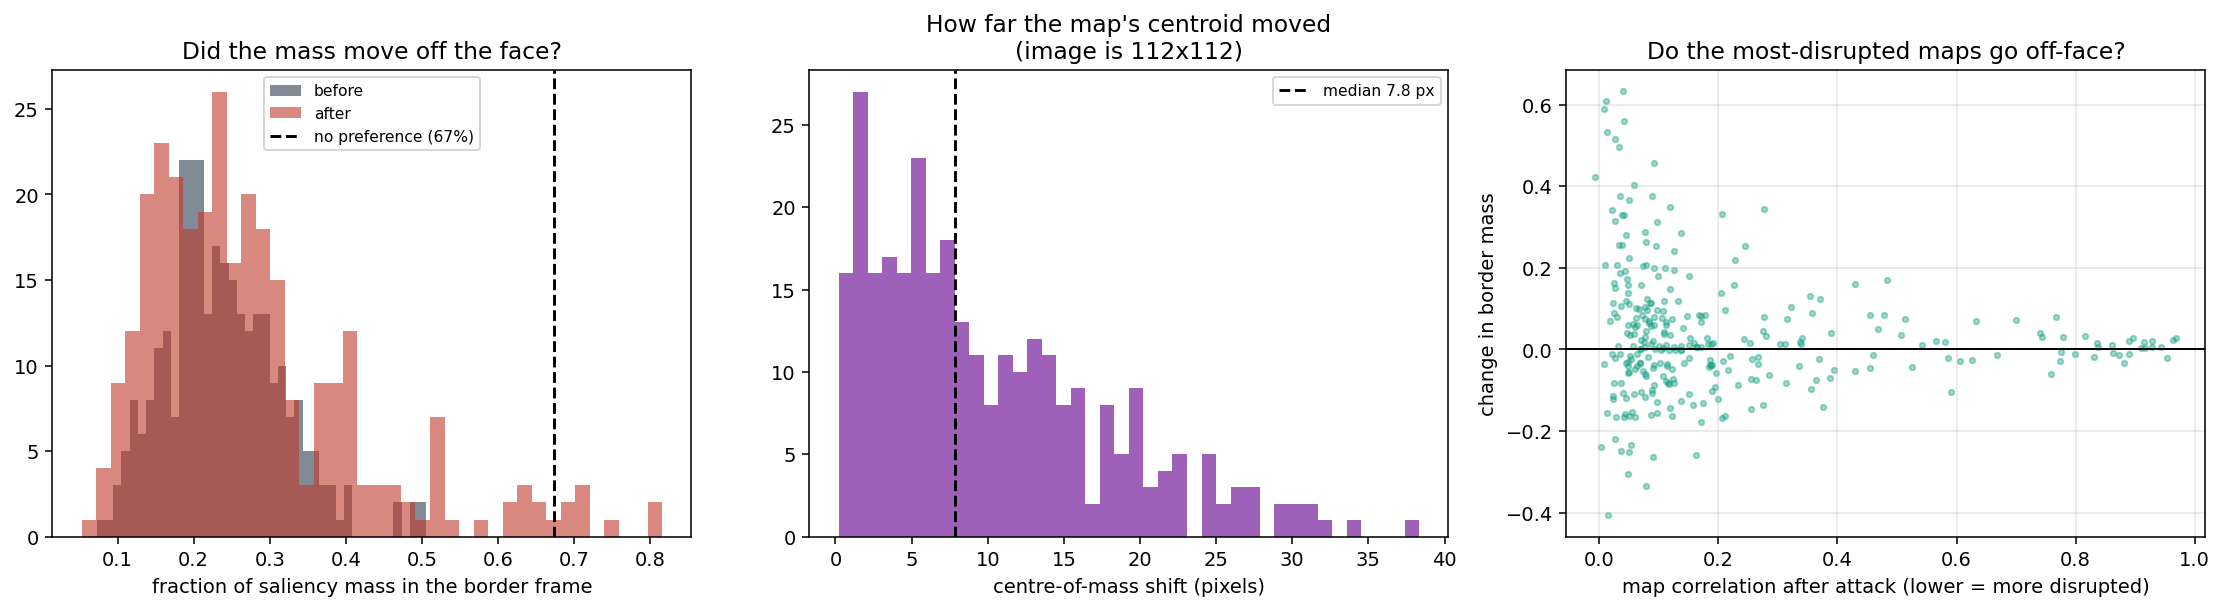
\includegraphics[width=\columnwidth]{11_relocation.png}
  \caption{Where the saliency mass went. Left: the distribution of off-face mass barely shifts
  under attack and stays far below the no-preference line. Middle: the centre of mass moves a
  median of 7.8\,px on a 112\,px image. Right: even the most-disrupted maps do not
  systematically push mass off the face. Measured under the wider border-frame definition.}
  \label{fig:relocation}
\end{figure}

\begin{figure}[!t]
  \centering
  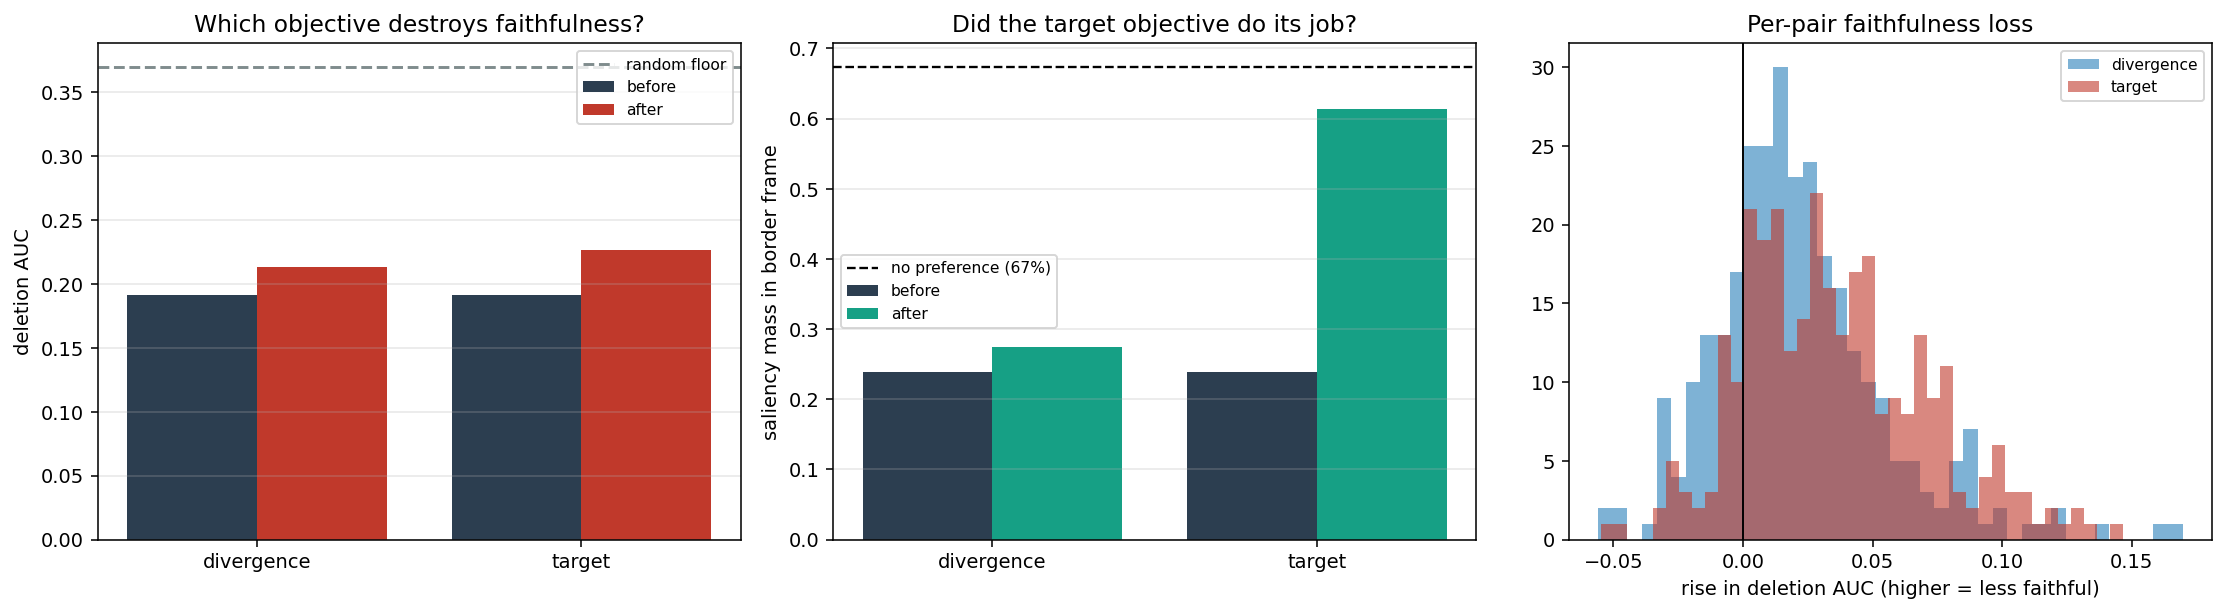
\includegraphics[width=\columnwidth]{11_target_mode.png}
  \caption{Target objective against decorrelation. Left: both objectives lift the deletion
  AUC, the target objective further, but neither reaches the random floor. Middle: the target
  objective does succeed at its own task, as off-face saliency mass rises sharply. Right: the
  per-pair distribution of faithfulness lost is shifted right for the target objective.
  Border-frame definition; the ellipse result is in Table~\ref{tab:targetmode}.}
  \label{fig:targetmode}
\end{figure}

\begin{figure}[!t]
  \centering
  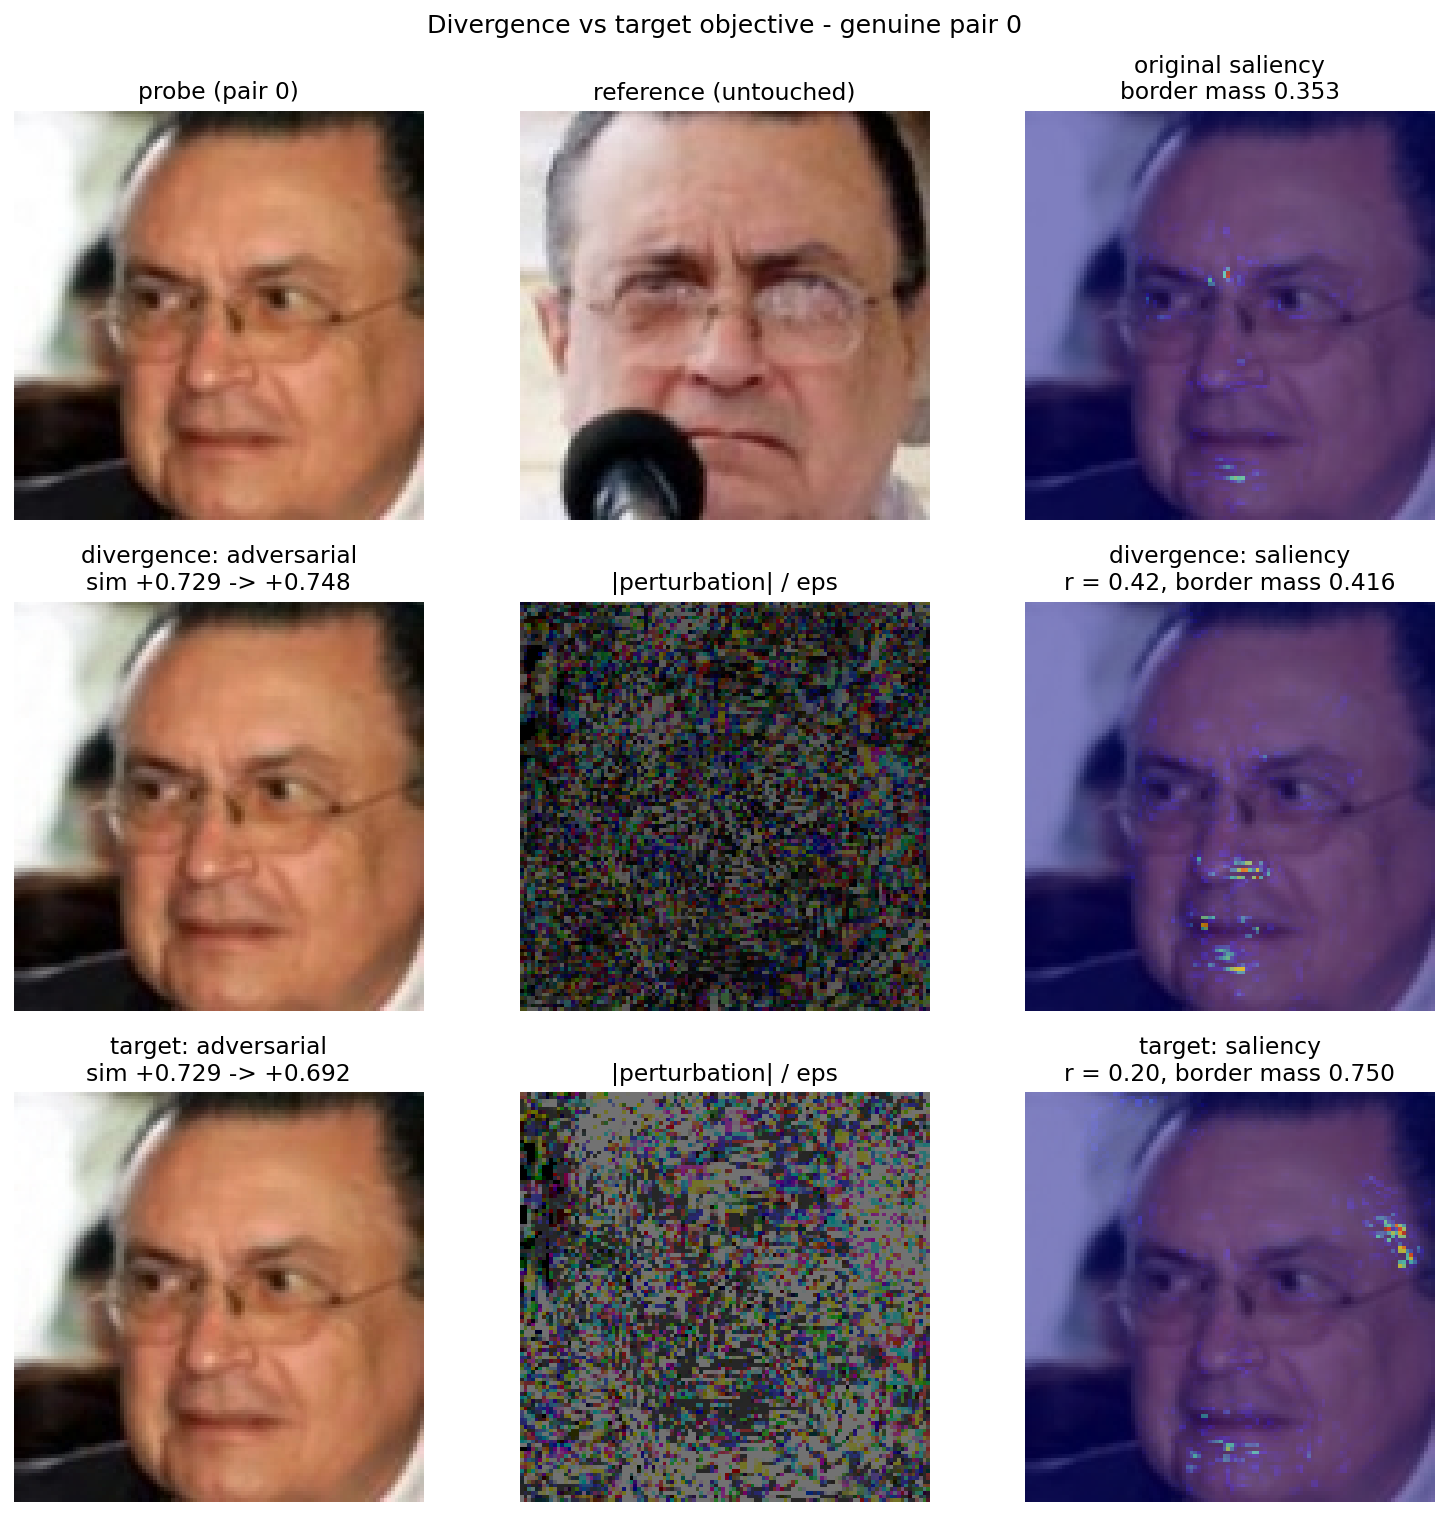
\includegraphics[width=0.86\columnwidth]{11_modes_pair0.png}
  \caption{The two objectives on the same pair. Under \texttt{divergence} (middle row) the
  saliency relocates from the eyes to the mouth and chin, still on the face. Under
  \texttt{target} (bottom row) a visible cluster appears in the upper-right background and
  off-face mass more than doubles. Both leave the photograph unchanged to the eye and the
  score within the band ($+0.729 \rightarrow +0.748$ and $+0.692$). This is redundancy and
  invariance in one picture: the attack can move mass, but what it moves it \emph{onto} still
  has to be somewhere the model looks.}
  \label{fig:modespair}
\end{figure}

\end{document}
